% Full instructions available at:
% https://github.com/elauksap/focus-beamertheme

\newcommand*\circled[1]{\tikz[baseline=(char.base)]{
            \node[shape=circle,draw,inner sep=2pt] (char) {#1};}}

\documentclass{beamer}
\usetheme{focus}

\title{GUIDA SICURA: Cap. Z}
\subtitle{uso ed equipaggiamento del veicolo}
\author{ACI Prima Porta}
\date{}
\titlegraphic{\vspace{1cm}
    
\includegraphics[scale=0.89]{images/logo.jpg}
}

\begin{document}
    \begin{frame}
        \maketitle
    \end{frame}
    
   % \begin{frame}{overview}
    %    \tableofcontents
    %\end{frame}
    
 %   \section{Introduction}
    
    \begin{frame}{Ho comprato una macchina nuova?}
    Che fare? Che documenti servono?
    
    \begin{figure}[ht!]
    \centering
         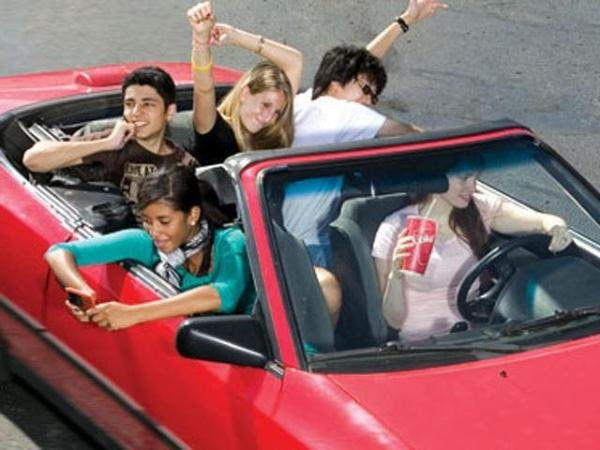
\includegraphics[width = 8cm]{images/new_car.jpg}
    \end{figure}
      \end{frame}
      
     \begin{frame}{Adempimenti}
         \transdissolve
         \begin{figure}[ht!]
    \centering
         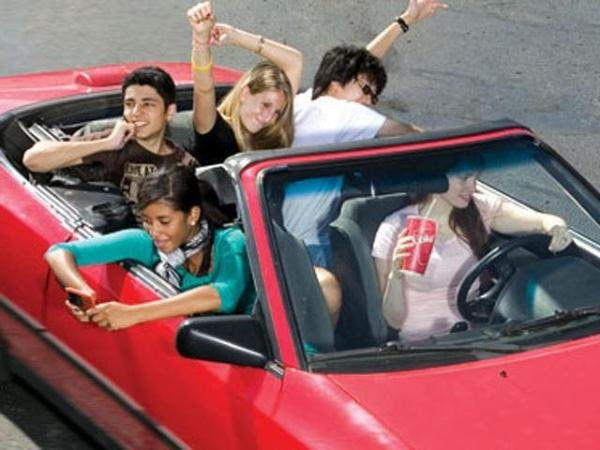
\includegraphics[width = 3cm]{images/new_car.jpg}
    \end{figure}
    Vai all'ACI di Prima Porta da Andrea: 
    \begin{enumerate}
    \item<2-> PATENTE 
    \item<3-> IMMATRICOLAZIONE
    \item<4-> ASSICURAZIONE
    \end{enumerate}
        
        \only<2>{\begin{block}{PATENTE}
        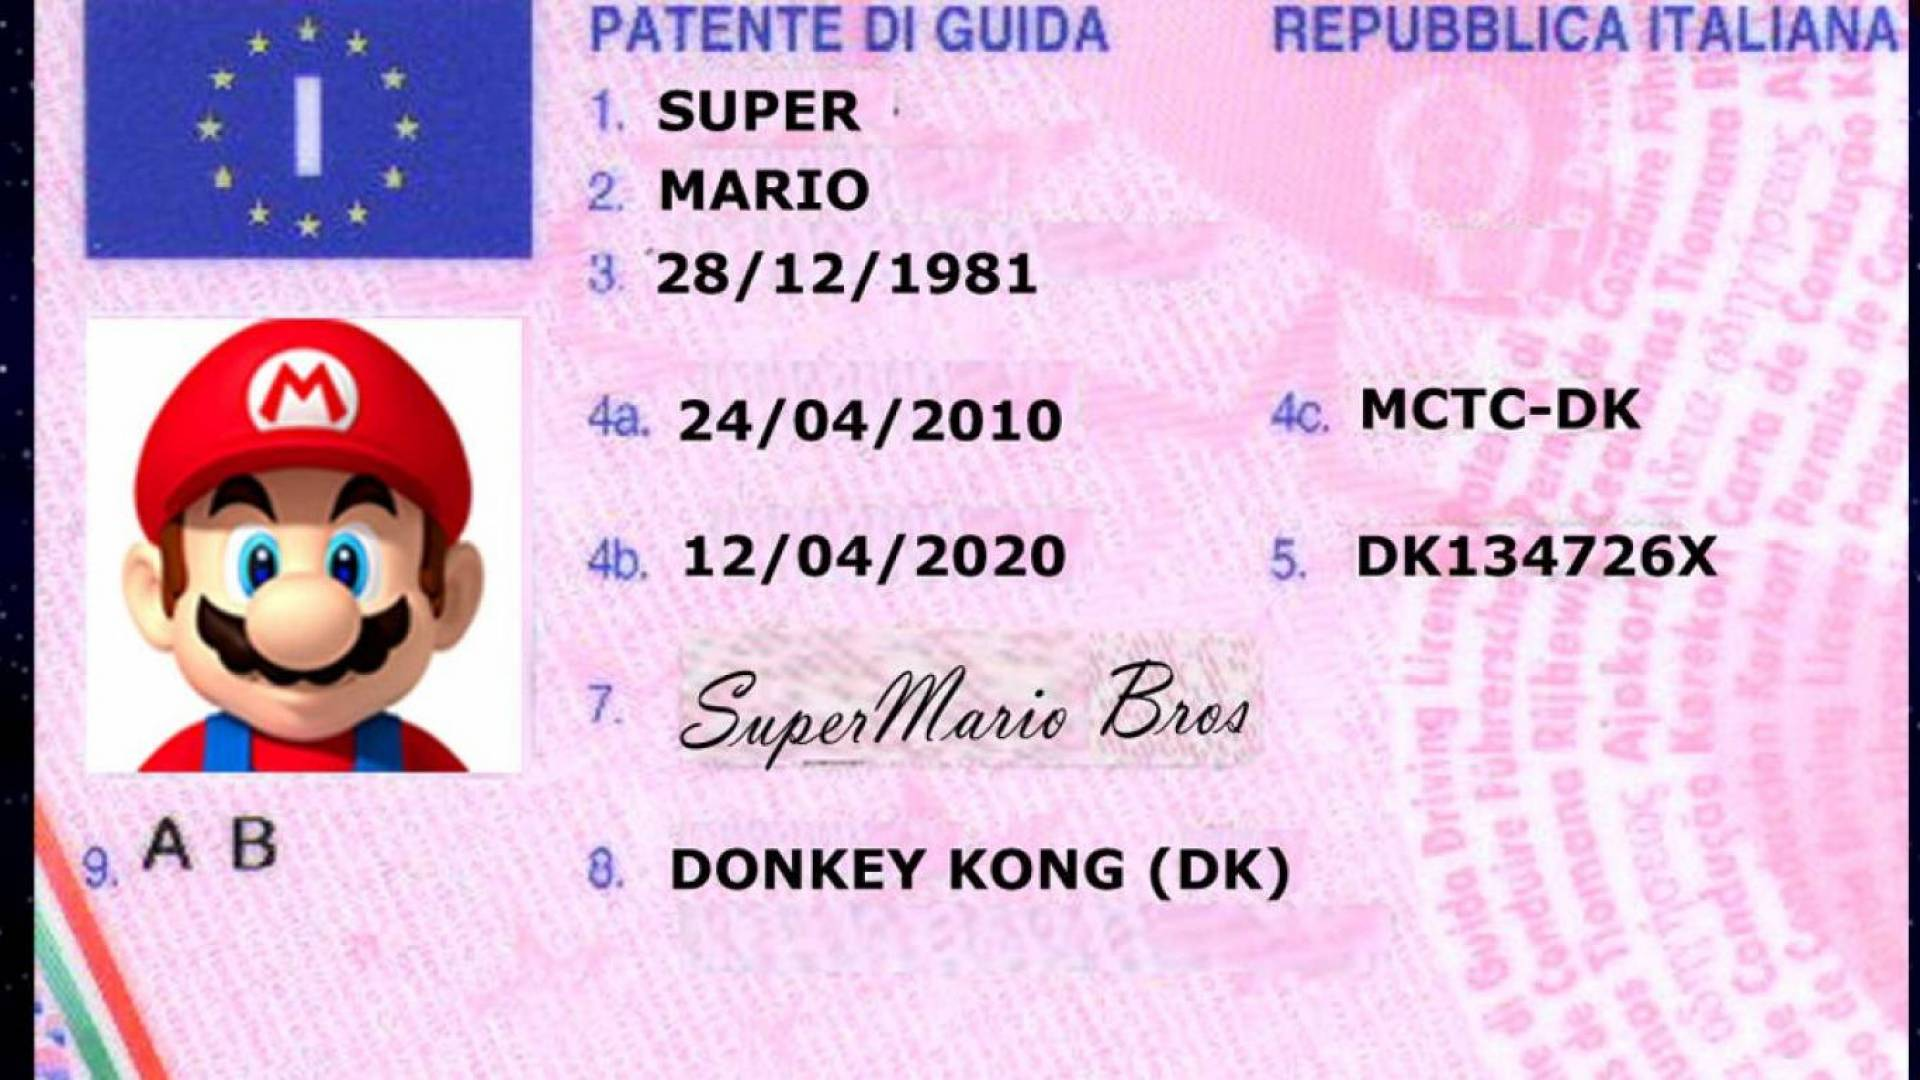
\includegraphics[width = 3cm]{images/patente.jpg}
        \end{block}}
        
        \only<3>{\begin{block}{ targhe + carta di circolazione}
         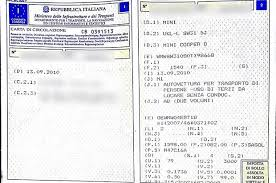
\includegraphics[width = 3cm]{images/libretto.jpg}
          
\includegraphics[width = 3cm]{images/targa.jpg}
          \end{block}
          }
            \only<4>{\begin{block}{ASSICURAZIONE}
         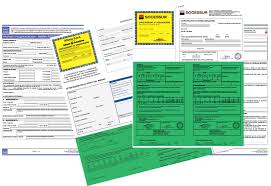
\includegraphics[width = 3cm]{images/assicurazione.jpg}
          \end{block}
          }
     \end{frame}
     
     
     \begin{frame}{Quiz}
     E' di norma \only<2->{\alert{di norma}} vietato condurre sulle strade pubbliche un autoveicolo non immatricolato
     
     \begin{center}
     \only<1>{\Huge{\circled{V}} \Huge{\circled{F}}}
        \only<2->{\Huge{\color{green}{\circled{V}}} \Huge{\circled{F}}}
     \end{center}
         
     \end{frame}
    

\end{document}
